\ProjectChapter{How to Use These Notes}{guide:reader}
A structural engineer opens a finite-element package and finds that its solver was written
in Fortran and C++. A process engineer inherits a spreadsheet full of VBA macros. A test
bench in the laboratory runs MATLAB scripts, the controller on the production line is
programmed in a language called Structured Text, and the dashboard that displays the plant
data is written in JavaScript. All of them learned to program in one language, and all of
them now have to read several.

You are learning to program in \py. That is the right first language for an engineer in
2026: it is free, readable, and used everywhere from data analysis in a chemical plant to
the control software of a research robot. These notes are a map of the other languages you
will meet. They do not replace the \py lectures and laboratories; read them alongside.
Each chapter introduces one language or a family of related languages: where it came
from, what engineers use it for, how to write and run a first program, how its basic
building blocks look, and what it is good and bad at. Every language chapter solves the
same small engineering problem, so that you can compare the languages line by line.

The title, \emph{From Formulas to Programs}, names what all these languages are for. An
engineer starts with a formula or a physical law and needs a program that computes with
it. Fortran, the oldest language in these notes, took its name from exactly this step:
\emph{formula translation}. The \hyperref[epilogue]{Epilogue} follows that idea from 1957
to the present and beyond.

\section*{Why learn about several languages?}

You will write most of your code in one or two languages. So why read about ten?
There are three practical reasons.

\begin{enumerate}
\item \textbf{You will read more code than you write.} Engineers inherit code:
  a Fortran solver from the 1990s, a MATLAB toolbox from a former student,
  a C driver for a sensor. Being able to read such code, even slowly, and
  recognise what it does is a real professional skill.
\item \textbf{Concepts transfer; syntax does not matter much.} Variables, loops,
  functions, arrays and files exist in every language. Once you see the same idea
  written five ways, you understand the idea, not just the \py spelling of it.
  This makes your \py better, too.
\item \textbf{Choosing the right tool is an engineering decision.} A spreadsheet
  macro, a \py script and a C++ program can all compute a heat-exchanger
  design. Which one you should choose depends on who will use it, how fast it must
  run, how long it must live and what hardware it runs on. You can only make that
  choice if you know the options.
\end{enumerate}

\section*{Choose a starting point}
\textbf{If you read only part of these notes.} Read Chapters 1--3, Chapter 16 and the
Epilogue carefully. Use Chapters 4--15 as a map: read them to recognise each language and
what it is for, not to memorise its syntax.
\par\textbf{Start with the foundations (Chapters 1--2).} Chapter~\ref{ch:intro} explains what a
programming language is and how languages differ. Chapter~\ref{ch:howcoderuns} explains how
code is turned into something a computer can execute, and how numbers are stored. Both
prepare you for everything that follows.
\par\textbf{Study \py carefully (Chapter 3).} Chapter~\ref{ch:python} is the longest
chapter and follows the order of topics in the course. Use it to revise.
\par\textbf{Read the other language chapters for orientation (Chapters 4--14).} You do not
need to memorise their syntax. Read each one with a question in mind: \emph{how is this
language different from \py, and why?} The exercises can be done with free tools.
\par\textbf{Compare and choose (Chapters 15--16).} Chapter~\ref{ch:rosetta} solves the same
three tasks in thirteen languages side by side. Chapter~\ref{ch:choosing} discusses how to
choose a language and how to write code that others can trust. The Epilogue closes with
the history and the likely future of the languages of engineering.
\par\textbf{Type the examples.} Reading code is good; running and changing it is much
better. Every complete program in these notes is short enough to type in a few minutes,
and all of them are in the \file{code} folder of the repository named at the end of this
guide.

\section*{Read the page}
A complete program is printed with its file name and with line numbers:
\begin{lstlisting}[language=Python,style=numbered,title={\footnotesize\sffamily\bfseries\color{accent}\texttt{python/hello.py}\normalfont\sffamily\color{muted}\enspace a first script}]
print("Hello, engineers!")
\end{lstlisting}
What the program prints follows on a pale blue panel with a blue bar at the left. It is
the real output of the program, not a retyped copy:
\begin{lstlisting}[style=output,title={\footnotesize\sffamily\color{muted}Output}]
Hello, engineers!
\end{lstlisting}
Commands that you type into a terminal (the ``command line'') are shown on a dark panel.
The \texttt{\$} sign is the prompt; do not type it.
\begin{lstlisting}[style=shell]
$ python3 hello.py
\end{lstlisting}
These commands are written for Linux and macOS. On Windows, use the Windows Subsystem for
Linux (WSL) or one of the browser-based options; both are explained in the guide
\hyperref[app:install]{Installing and Running the Languages} at the back.
Short fragments inside the text have a frame but no file name. They illustrate one point
and may need surrounding code before they run.

Boxed notes come in five colours:
\begin{keyidea}
A concept to understand and remember.
\end{keyidea}
\begin{engnote}
How the topic matters in real engineering work.
\end{engnote}
\begin{pitfall}
A mistake that beginners, and experienced programmers, often make.
\end{pitfall}
\begin{history}
Where a language or an idea came from.
\end{history}
\begin{tryit}
A short activity to do at the computer.
\end{tryit}
Each chapter ends with exercises under the heading \emph{Try it yourself}. Hints and
answers to selected exercises are at the back; click an exercise number there to jump
back to the question.

\section*{Follow one example through every language}
\label{sec:runningexample}

To compare languages fairly we will solve the same problem in each of them. The problem
is one you know from Newtonian mechanics. A skydiver of mass $m$ falls from rest.
Gravity pulls down with force $mg$; air resistance pushes up with a force that grows
with the square of the speed, $c v^2$, where $c$ is a drag coefficient (in kg/m).
Newton's second law gives
\begin{equation}
  m\frac{dv}{dt} = mg - c v^2, \qquad v(0) = 0.
  \label{eq:drag}
\end{equation}
When the two forces balance, the acceleration is zero and the speed stops growing.
This \emph{terminal velocity} is
\begin{equation}
  v_\mathrm{t} = \sqrt{\frac{mg}{c}}.
  \label{eq:vterminal}
\end{equation}
Equation~\eqref{eq:drag} happens to have an exact solution,
\begin{equation}
  v(t) = v_\mathrm{t}\tanh\!\left(\frac{g t}{v_\mathrm{t}}\right),
  \label{eq:dragexact}
\end{equation}
which lets us check a numerical answer. The numerical method we use is the simplest one
there is, the \emph{explicit Euler method}. We replace the derivative by a finite
difference over a small time step $\Delta t$:
\begin{equation}
  \frac{v_{n+1} - v_n}{\Delta t} \approx g - \frac{c}{m} v_n^2
  \quad\Longrightarrow\quad
  v_{n+1} = v_n + \Delta t\left(g - \frac{c}{m}v_n^2\right).
  \label{eq:euler}
\end{equation}
Starting from $v_0 = 0$ we apply this update again and again. Each application moves
time forward by $\Delta t$. In every language chapter we use the same numbers:
$m = 80\unit{kg}$, $c = 0.25\unit{kg/m}$, $g = 9.81\unit{m/s^2}$, a time step
$\Delta t = 0.5\unit{s}$, and we stop at $t = 20\unit{s}$. With these numbers
$v_\mathrm{t} = \sqrt{80 \times 9.81/0.25} \approx 56.03\unit{m/s}$.

The program in each language does four things that almost every engineering program does:
\begin{enumerate}
\item it stores some \textbf{parameters} in variables;
\item it defines a \textbf{function} (the right-hand side $g - (c/m)v^2$);
\item it uses a \textbf{loop} to step forward in time and stores the results in an
  \textbf{array};
\item it \textbf{prints} a formatted table and compares with the exact answer.
\end{enumerate}
Figure~\ref{fig:dragresult} shows the result. You will see this curve many times.

\begin{figure}[htbp]
\centering
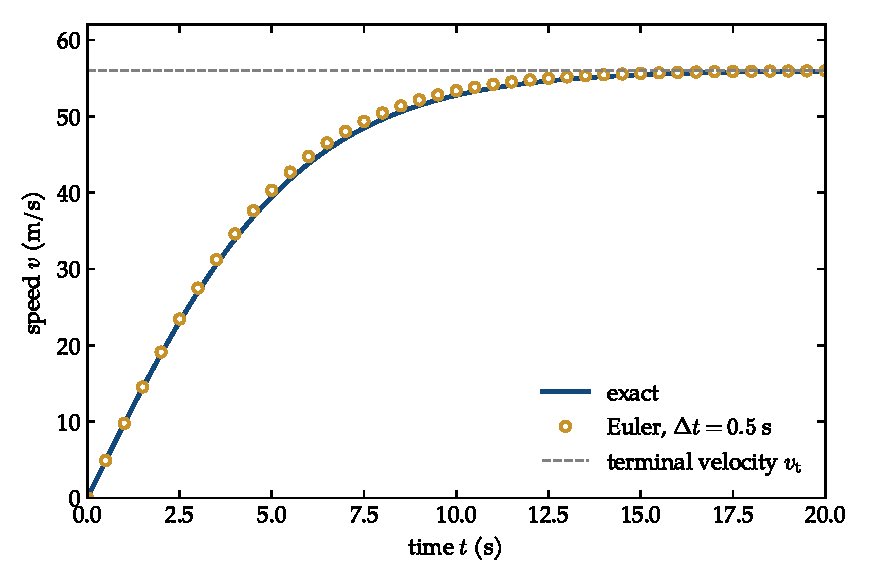
\includegraphics[width=0.72\linewidth]{figures/drag_euler.pdf}
\caption[{The running example}]{The running example. Speed of a falling skydiver with quadratic air drag ($m=80\unit{kg}$,
$c=0.25\unit{kg/m}$). The solid line is the exact solution~\eqref{eq:dragexact};
the markers are the Euler method with $\Delta t = 0.5\unit{s}$. The dashed line is the
terminal velocity. Every language chapter reproduces this calculation.}
\label{fig:dragresult}
\end{figure}

\section*{About these notes}
Reading notes for ENG 101 Programming for Engineers (6 ECTS), Nazarbayev University, Fall
2026. Version 1.0.1, 18 November 2026; corrections are
listed in the file \file{ERRATA.md} of the repository. \copyright\ 2026 Yanwei Wang. The notes are provided to students of ENG 101 for study.
MATLAB examples were tested in GNU Octave, which runs the same core language, and the
C\# examples with the Mono compiler. The Wolfram Language programs were run in
Mathematica and the Julia programs in Julia 1.13. Only the short fragments in
Chapter~\ref{ch:others} (VBA, Structured Text, Verilog, VHDL, Modelica, G-code), which need
special tools, were checked by hand and were not run. The data files used in the examples
contain invented teaching values, not measurements. All programs, data files and the
source of these notes are at \url{https://github.com/ktwyw/from-formulas-to-programs};
the script \file{tools/check\_examples.py} there re-runs every program and compares its
output with the output printed in these notes. Contact:
\texttt{yanwei.wang@nu.edu.kz}; ORCID 0000-0002-8488-9833.

\section*{Acknowledgements}
These notes grew out of questions asked by ENG 101 students: \emph{``Why do we learn
\py and not C?''}, \emph{``Is MATLAB still used?''}, \emph{``What language does my
calculator use?''}. Thank you for asking them. Comments, corrections and suggestions are
very welcome; please send them by email.

\par\medskip\hfill Yanwei Wang, Astana, November 2026
